\documentclass[orivec]{llncs}

\usepackage{algorithm, algpseudocode}
\usepackage{amssymb}
\usepackage{amsmath}
\usepackage{graphicx}
\usepackage{epsfig}
%\usepackage{subfigure}
\usepackage{listings}
\usepackage{verbatim}
\usepackage{stmaryrd}
\usepackage[utf8]{inputenc}
\usepackage[T1]{fontenc} 
\usepackage[hyphens]{url}
\usepackage[caption=false]{subfig}
\usepackage{wrapfig}

\lstset{
numbers=left,
numberstyle=\tiny,
language={Java},
mathescape=true,
flexiblecolumns=true,
morekeywords={call,method,var,assert,share,unshare,acquire,release,fork,join,free,invariant,requires,ensures,acc,rd,old},
basicstyle=\sffamily\scriptsize,
moredelim=[is][\itshape]{@}{@},
stepnumber=1,
numbersep=2pt,
numbers=none}

\urldef{\mailpietro}\path|pietro.ferrara@inf.ethz.ch|   
\urldef{\mailgiuseppe}\path|maggiore.g@nhtv.nl|   
\urldef{\mailgiuliatino}\path|{costantini, cortesi}@dsi.unive.it|    
\newcommand{\keywords}[1]{\par\addvspace\baselineskip
\noindent\keywordname\enspace\ignorespaces#1}

\makeatletter 
\newcommand*\sbigtimes{\mathop{\mathpalette\@sbigtimes\relax}\displaylimits} 
\newcommand*\@sbigtimes[2]{% 
  \vcenter{\hbox{\sffamily\@nameuse{\string#1bt}X}}\vphantom{\prod}} 
\@namedef{\string\displaystyle bt}{\huge} 
\@namedef{\string\textstyle bt}{\Large} 
\@namedef{\string\scriptstyle bt}{\small} 
\@namedef{\string\scriptscriptstyle bt}{\footnotesize} 
\makeatother

\pagestyle{plain}

\newcommand{\Sample}{\ensuremath{\mathsf{Sample}}}

%\newcommand{\todo}[1]{\textbf{TODO:#1}}
%\newcommand{\commentpietro}[1]{\textbf{Pietro says: } \textit{#1}}
%\newcommand{\commentgiulia}[1]{\textbf{Giulia says: } \textit{#1}}
\newcommand{\todogiulia}[1]{\footnote{\textbf{Todo GIULIA: #1}}}
\newcommand{\todopietro}[1]{\footnote{\textbf{Todo PIETRO: #1}}}
%\newcommand{\todogiuseppe}[1]{\footnote{\textbf{Todo GIUSEPPE: #1}}}
\newcommand{\goodgap}{\hspace{1.536pt}}


\newcommand{\Java}{\ensuremath{\mathsf{Java}}}
\newcommand{\real}{\ensuremath{\mathbb{R}}}
\newcommand{\integer}{\ensuremath{\mathbb{Z}}}
\newcommand{\naturals}{\ensuremath{\mathbb{N}}}
\newcommand{\Scala}{\ensuremath{\mathsf{Scala}}}
\newcommand{\IVSF}{\ensuremath{\mathsf{IVSF}}}
\newcommand{\TSF}{\ensuremath{\mathsf{TSF}}}
\newcommand{\CSharp}{\ensuremath{\mathsf{C\#}}}
\newcommand{\FSharp}{\ensuremath{\mathsf{F\#}}}

\newcommand{\variables}{\ensuremath{\mathsf{Vars}}}

\newcommand{\lfp}[2]{\ensuremath{\mathit{lfp}^{#1}_{#2} \hspace{2pt}}}
\newcommand{\parts}[1]{\ensuremath{\wp(#1)}}
\newcommand{\dom}[1]{\ensuremath{\cfunction{dom}(#1)}}
\newcommand{\statement}[1]{\ensuremath{\mathtt{#1}}}
\newcommand{\funzione}[2]{\ensuremath{#1 \rightarrow#2}}
\newcommand{\pair}[2]{\ensuremath{#1 \times #2}}
\newcommand{\cartesianproduct}[2]{\ensuremath{#1 \times #2}}
\newcommand{\reducedproduct}[2]{\ensuremath{#1 \varotimes #2}}
\newcommand{\true}{\cel{true}}
\newcommand{\false}{\cel{false}}
\newcommand{\booltop}{\cel{\top_B}}
\newcommand{\reducefunction}{\afunction{red}}
\newcommand{\gettype}{\afunction{getType}}
\newcommand{\getstatictype}[1]{\cfunction{\sttype}(#1)}
\newcommand{\sttype}{statictype}
\newcommand{\abstractn}{abstract}
\newcommand{\abstractfunction}[1]{\afunction{\abstractn}(#1)}


\newcommand{\sequence}[1]{\ensuremath{#1^*}}
\newcommand{\sem}[1]{\ensuremath{\llbracket \mathtt{#1} \rrbracket}}
\newcommand{\semanticanome}[1]{\ensuremath{\mathbb{#1}}}
\newcommand{\semantica}[2]{\ensuremath{\semanticanome{#1}\sem{#2}}}

%Concreto

%Dominio e semantica concrete
\newcommand{\cset}[1]{\ensuremath{\mathsf{#1}}}
\newcommand{\ctrace}[1]{\ensuremath{\trace{{\cset{#1}}}}}
\newcommand{\cel}[1]{\ensuremath{\mathsf{#1}}}
\newcommand{\cjoin}{\ensuremath{\cup}}
\newcommand{\cmeet}{\ensuremath{\cap}}
\newcommand{\corder}{\ensuremath{\subseteq}}
\newcommand{\cbot}{\ensuremath{\emptyset}}
\newcommand{\ctop}[1]{\cset{#1}}
\newcommand{\cfunction}[1]{\ensuremath{\mathit{#1}}}
\newcommand{\csemantics}[2]{\ensuremath{\semantica{#1}{#2}}}

%Astratto

%Dominio e semantica astratte
\newcommand{\adomain}{\ensuremath{\mathcal{H}}} % D^\sharp}}
\newcommand{\aset}[1]{\cset{\overline{#1}}}
\newcommand{\ael}[1]{\cel{\overline{#1}}}
\newcommand{\alub}{\ensuremath{\cup^\mathcal{H} }} %\sharp}}
\newcommand{\aglb}{\ensuremath{\cap^\mathcal{H} }} %\sharp}}
\newcommand{\awidening}{\ensuremath{\nabla_{\mathcal{H} }}} %D^\sharp}}}
\newcommand{\aorder}{\ensuremath{\subseteq^\mathcal{H}}} %\sharp}}
\newcommand{\abot}{\ensuremath{\bot^\mathcal{H} }} %\sharp}}
\newcommand{\abtop}{\ensuremath{\top^\mathcal{H} }} %\sharp}}
\newcommand{\asemantics}[2]{\semantica{\afunction{\semanticanome{#1}}}{#2}}
\newcommand{\atrace}[1]{\ensuremath{\trace{#1}}}
\newcommand{\afunction}[1]{\ensuremath{\overline{\mathit{#1}}}}
\newcommand{\function}[1]{\ensuremath{\mathit{#1}}}
\newcommand{\agenericdomain}{\ensuremath{\mathcal{A}}}

\newcommand{\gas}{\ensuremath{\cset{\mathcal{REMOVE}}}}
%\newcommand{\hypercubes}{\ensuremath{\cset{\mathcal{H}}}}


\newcommand{\avaluename}{\ensuremath{\afunction{value}}}
\newcommand{\avalue}[1]{\ensuremath{\avaluename(#1)}}

\newcommand{\avariableindexname}{\ensuremath{\function{varIndex}}}
\newcommand{\avariableindex}[1]{\ensuremath{\avariableindexname(#1)}}
\newcommand{\aval}{\ensuremath{\cset{Val}}}


\title{The Domain of Parametric Hypercubes for Static Analysis of Computer Games Software}
%\subtitle{An efficient and disjunctive static analysis of physics simulations}

\author{Giulia Costantini\inst{1} \and Pietro Ferrara\inst{2} \and Giuseppe Maggiore \inst{3} \and Agostino Cortesi\inst{1}}

\institute{University Ca' Foscari of Venice, Italy\\\mailgiuliatino \and ETH Zurich, Switzerland\\\mailpietro \and IGAD, NHTV University of Breda, The Netherlands\\\mailgiuseppe}

\begin{document}

\maketitle

\begin{abstract}
Application domains like Computer Games Software are an interesting workbench to stress the trade-off between accuracy and efficiency of abstract domains for static analysis, in the Abstract Interpretation framework. Game software deeply relies on physics simulations, which are particularly demanding: due to the large amount of interleaving floating point variables, the numerical domains already studied in the literature either lack accuracy too much, or their use becomes unfeasible due to the exponential cost of abstract operations.

In this paper, we discuss the domain of Parametric Hypercubes, a novel disjunctive non-relational abstract domain. Its main features are: (i) it combines the low computational cost of operations on (selected) multidimensional intervals with the accuracy provided by lifting to a power-set disjunctive domain, (ii) the compact representation of its elements allows to limit the space complexity of the analysis, and (iii) the parametric nature of the domain provides a way to tune the accuracy/efficiency of the analysis by just setting the widths of the hypercubes sides.

The first experimental results on a representative Computer Games case study outline both the efficiency and the precision of the proposal.


\end{abstract}

\section{Introduction}
\label{sec:introduction}
Computer Games Software is a fast growing industry, with more than 200 million units sold every year, and annual revenue of more than 10 billion dollars. According to the Entertainment Software Association (ESA), more than 25\% of the software played concerns sport, action, and strategy games, where physics simulations are the core of the product, and compile-time verification of behavioural properties is particularly challenging for developers. 

The difficulty arises because, usually, these programs feature (i) a \statement{while} loop which goes on endlessly, (ii) a complex state made up by multiple real-valued variables, and (iii) strong dependencies among variables. 
Most of the times, a simulation consists in the initialization of the state (i.e., the variables which compose the simulated world) followed by an infinite \statement{while} loop which computes the numerical integration over time (i.e., the inductive step of the simulation). Such loop is executed until the game is stopped.
In addition, the variables of a physics simulation are real-valued, because they represent continuous values that map directly to physical aspects of the real world, like positions, velocities (speed plus direction), and accelerations. 
Finally, the variables of a simulation are strongly inter-related, because the simulation often makes decisions based on the values of particular variables. For example, the velocity of an object changes abruptly when there is a collision, which depends on the object position. Similarly, the position changes accordingly to the velocity, which in turn depends on the acceleration which may derive from the position (for a gravitational field) or from other parameters. 

Interesting properties on physical programs are, for example, the insurance that a rocket reaches a stable orbit, or that a bouncing ball arrives at a certain destination. To prove such properties statically, we need to precisely track relationships between variables. However, traditional approaches to static analysis are not best suited to deal with these kind of properties. On the one hand, non-relational domains 
%guarantee efficient analyses, but they 
are usually too approximate. On the other hand, the computational cost of sophisticated relational domains like Polyhedra \cite{CH78} or Parallelotopes \cite{AS12} is too high, and their practical use in this context becomes unfeasible.   

In this paper, we introduce Parametric Hypercubes, a novel disjunctive non-relational abstract domain. Its main features are: (i) it combines the low computational cost of operations on (selected) multidimensional intervals with the accuracy provided by lifting to a power-set domain, (ii) the compact representation of its elements allows to limit the space complexity of the analysis, and (iii) the parametric nature of the domain provides a way to tune the trade-off between accuracy and efficiency of the analysis by just setting the widths of the hypercubes sides. The domain can be seen as the combination of a suite of well-known techniques for numerical abstract domain design, like disjunctive powerset, and conditional partitioning. The most interesting points of our work are: (i) the approach: the design of the domain has as starting point the features of the application domains, (ii) the self-adaptive parameterization: a recursive algorithm is applied to refine the initial set of parameters in order to improve the accuracy of the analysis without sacrificing the performance, and (iii) the novel notion of \textquotedblleft offset\textquotedblright\ that allows to narrow the lack of precision due to the fixed width of intervals.
The analysis has been implemented, and it shows promising results in terms both of efficiency and precision when applied to a representative case study of Computer Games Software. 
%Also, we expect that our technique is generic enough to be successfully applied to other kinds of programs: an example is presented in Section \ref{sec:otherapplications}.

The rest of the paper is structured as follows. Section \ref{sec:syntax} presents the language syntax supported by our analysis and Section \ref{sec:case_study} introduces the case study which we use to experiment with our approach. Sections \ref{sec:hyper_cubes_domain} and \ref{sec:semantics} formally define the abstract domain and semantics, respectively. %Section \ref{sec:tuning} shows how to improve the performance and precision of the analysis. 
Section \ref{sec:experimental} contains the experimental results of our analysis applied to the case study of Section \ref{sec:case_study}. Section \ref{sec:related} presents the related work and Section \ref{sec:conclusions} concludes.



\section{Language syntax} \label{sec:syntax}
Let $\mathcal{V}$ be a finite set of variables, and $\mathcal{I}$ the set of all real-valued intervals. Figure \ref{fig:syntax} defines the language.
We focus on programs dealing with mathematical computations over real-valued variables. Therefore, we consider expressions built through the most common mathematical operators (sum, subtraction, multiplication, and division). An arithmetic expression can be a constant value ($c \in \real$), a non-deterministic value in an interval ($I \in \mathcal{I}$), or a variable ($V \in \mathcal{V}$). We also consider boolean conditions built through the comparison of two arithmetic expressions. Boolean conditions can be combined as usual with logical operators (and, or, not). As for statements, we support the assignment of an expression to a variable, \statement{if-then-else}, \statement{while} loops, and concatenation. 
Even though this syntax is simple and limited, many physical simulations can be built through it \cite{B12}, since their complexity lies mostly in their logic and not in the used constructs.

\begin{figure}
\vspace{-15pt}
$$V \in \mathcal{V}, I \in \mathcal{I}, c \in \real$$
$$E :=  c | I | V | E\ <aop>\ E \textrm{ where }<aop> \in \{+, -, \times, \div \}$$
$$B := E <bop> E | B\ and\ B | not\ B | B\ or\ B \textrm{ where } <bop> \in \{\geq, >, \leq, <, \neq \}$$
$$P := V = E | \statement{if}(B)\ \statement{then}\ P\ \statement{else}\ P | \statement{while}(B)\ P | P;P $$
\caption{Syntax}
\label{fig:syntax}
\end{figure}
\vspace{-20pt}

\section{The case study of bouncing balls}
\label{sec:case_study}
As a case study, consider a program which generates a bouncing ball on the screen. The ball starts at the left side of the screen (even though the exact starting position is not fixed), and it has a random initial velocity. The horizontal direction of the ball is always towards the right of the screen, since the horizontal component of the velocity is always positive. Whenever the ball reaches the \textquotedblleft ground\textquotedblright\ (i.e., the bottom of the screen), it bounces (i.e., its vertical velocity is inverted). When the ball reaches the right border of the screen, it disappears. We want to verify that $T$ seconds after the generation of the ball, such ball has already exited from the screen (we call this property \emph{Property 1}). The code of the program which simulates the creation and movement of the ball is reported in Listing \ref{lst:casestudy}. 

\begin{lstlisting}[caption={Case study: bouncing-ball code},label={lst:casestudy}]
let px = rand(0.0, 10.0)
let py = rand(0.0, 50.0)
let vx = rand(0.0, 60.0)
let vy = rand(-30.0, -25.0)
let dt = 0.05
let g = -9.8
let k = 0.8

while (true) do
   if( py >= 0.0 ) then 
     (px, py) = (px + vx * dt, py + vy * dt)
     (vx, vy) = (vx, vy + g * dt)
   else
     (px, py) = (px + vx * dt, 0.0)
     (vx, vy) = (vx, -vy) * k
\end{lstlisting}

The structure of this program respects the generic structure of a physics simulation, as explained in Section \ref{sec:introduction}. In fact, it starts with the world initialization, that is, the assignment of the initial values to the program variables. The meanings of the variables are as follows:
\begin{itemize}
\item \statement{(px,py)} represents the current position of the ball in the screen. The initial position of the ball is generated randomly. We only know that the ball is generated in proximity of the left side of the screen (since the $x$-coordinate is between $0.0$ and a low value such as $10.0$).
\item \statement{(vx,vy)} represents the current velocity of the ball. The initial velocity is generated randomly as well. Note that the horizontal velocity is always positive, because we want to throw the ball towards the right of the screen. The vertical velocity, instead, is negative, because we throw the ball downwards.
\item \statement{dt} represents the time interval between iterations of the loop. This value is constant and known at compile time. We consider a simulation running at 20 frames per second: this means that $\statement{dt}=1/20=0.05$.
\item \statement{g} represents the force of gravity ($-9.8$).
\item \statement{k} represents how much the impact with the ground decreases the velocity of the ball.
\end{itemize}

The \statement{while} loop updates the world variables, that is, the ball position and velocity. In particular, if the ball is in the air (i.e., its vertical position is greater or equal to $0.0$), its position is updated according to the rule of uniform linear motion. The vertical velocity is also updated to take into account the force of gravity, while the horizontal one remains unmodified. Otherwise, the ball touches the ground\footnote{We must wait that the position of the ball is \emph{lower} than zero before making it bounce, otherwise a ball could bounce before having actually touched the ground. The ball could disappear from the screen for a bit, but, considering the frame-rate of modern games, this artifact is almost not perceived by the user.} and it bounces. To simulate the bouncing, we update the horizontal position as usual, and we force the vertical position to zero. Moreover, the vertical velocity is inverted (instead of going downwards, the ball must go upwards) and decreased, along with the horizontal velocity, through the constant factor \statement{k}, to consider the force which is lost in the impact with the ground. 

Verifying properties on this kind of programs can have interesting practical impact also on more complex programs, since it is a basic physics simulation which can be used in many contexts \cite{E10}. For instance, consider the case where some game entity discreetly generates bouncing balls on the screen. The interval between the creation of two balls is constant and known at compile time (let us call it \statement{creationInterval}). The pseudo code of the main method of this simulation is shown in Listing \ref{lst:casestudyExternal}, where \statement{updateBall(b)} is a function which updates the ball \statement{b} according to the physics of the simulation (i.e., the body of the while loop of Listing \ref{lst:casestudy}) and \statement{generateNewBall()} is a function which creates a new ball (with the values of the initialization of Listing \ref{lst:casestudy}).

\begin{lstlisting}[caption={Bouncing ball generation},label={lst:casestudyExternal}]
let balls = Set.empty
let dt = 0.05
let creationInterval = 3.0
let timeFromLastCreation = 0.0
while (true) do
	foreach ball in balls
		updateBall(ball)	
	if(timeFromLastCreation >= creationInterval)
		generateNewBall()
		timeFromLastCreation = 0.0
	else
		timeFromLastCreation += dt
\end{lstlisting}

If we verify \emph{Property 1} on Listing \ref{lst:casestudy}, we are sure that a single ball will have exited the screen after $T$ seconds. We also know that, in Listing \ref{lst:casestudyExternal}, we generate one ball each $\statement{creationInterval}$ seconds. This means that, having verified \emph{Property 1}, we can guarantee in Listing \ref{lst:casestudyExternal} that \emph{a maximum of $\lceil \frac{T}{\statement{creationInterval}} \rceil$ balls will be on the screen at the same time}. Such information is useful for performance reasons (crucial in a game), since each ball requires computations for its rendering and updating. 

%Thus, what we would like to prove is that \emph{there never are more than $N$ balls on the screen at the same time}. Since we know that we generate a ball at each \statement{creationInterval} seconds, this property is equivalent to verify that, $N \times \statement{creationInterval}$ seconds after the generation of a ball, such ball has already exited from the screen. In fact, we know that after such time ($N \times \statement{creationInterval}$ seconds), other $N$ balls will have been generated, so the first ball must have already exited. \footnote{This property is more restrictive than the original one, since the balls do not necessarily exit the screen in the same order they were created, depending on their random initial velocity. Anyway, the increased strictness means that, if we prove this property, we have also proven the original one.}

The theoretical interest of this case study lies in the fact that non-relational or non-disjunctive approaches are not properly suited to verify \emph{Property 1}. Consider for example the Interval domain where every variable of the program is associated to a single interval. After a few iterations, when the vertical position possibly goes to zero, the analysis is no more able to distinguish which branch of the \statement{if-then-else} to take. In this case, the lub operator makes the vertical velocity interval quite wider, since it will contain both positive and negative values. After that, the precision gets completely lost, since the velocity variable affects the position and vice-versa. On the other hand, the accuracy that would be ensured by using existing disjunctive domains has a computational cost that makes this approach unfeasible for practical use.



\section{The Parametric Hypercubes domain}
\label{sec:hyper_cubes_domain}
Intuitively, an abstract state of the Parametric Hypercubes domain (\adomain) tracks disjunctive information relying on floating-point intervals of fixed width. A state of \adomain\ is made by a set of hypercubes of dimension $|\variables|$. Each hypercube has $|\variables|$ sides, one for each variable, and each side contains an abstract non-relational value for the corresponding variable. Each hypercube represents a set of admissible combinations of values for all variables. 

The name Hypercubes comes from the geometric interpretation of the elements of \adomain . The concrete state of a program with variables in $\variables$ is an environment in $\funzione{\variables}{\real}$. This can be isomorphically represented by a tuple of values where each item of the tuple represents a program variable. Seen in this way, the concrete state corresponds, geometrically, to \emph{a point} in the $|\variables|$-dimensional space. 
%Each dimension of the space represents the possible values that the corresponding variable of the program can assume. The concrete trace of a program is a sequence of points in such space (one for each state of the trace). 
The hypercubes of our domain \adomain\ are \emph{volumes} in the same $|\variables|$-dimensional space. 
%Each side of the hypercube is the concretization of the abstract value of the corresponding variable, and thus it corresponds to a set of values in that dimension of the space. The concretization of an hypercube is the set of all the points contained in its volume. A state in \adomain\ is composed by a set of hypercubes: its concretization is the union of all the volumes of its hypercubes.  In this way we track disjunctive information.

\vspace{-10pt}
\subsection{Lattice structure}
\vspace{-5pt}
An abstract state of \adomain\ tracks a \emph{set} of hypercubes, and each hypercube is represented by a tuple of abstract values. The dimension of these tuples is equal to the number of program variables.
%: this means that each variable is associated to a given item of the tuple (i.e., to a specific side of the hypercube). 
%Consider for instance a program in which $\variables = \{x_1, x_2\}$. In this case, the hypercubes of \adomain\ are 2D-rectangles. In particular, the two sides of a single hypercube are two abstract values, one for $x_1$ and one for $x_2$.
%A priori, our approach is modular w.r.t. the non-relational abstract domain we adopt to approximate the values of single variables inside an hypercube.
We abstract floating-point variables through intervals of real values. A set of hypercubes allows us to track disjunctive information, and this is useful when the values of a variable are clustered in different ranges.
%: instead of having a very big interval to cover them all (and which would cover also a lot of invalid values), we use two (or more) smaller intervals. Since it would be particularly expensive to perform all the lattice operators pointwisely, we partition the possible values into intervals of fixed width. As an example, suppose that the initial vertical velocity of the balls of our case study ranges between $50.0$ and $60.0$ or between $-60.0$ and $-50.0$. A single interval would approximate these values with $[-60.0 .. 60.0]$, while with our approach we track two intervals, $[-60.0 .. -50.0]$ and $[50.0 .. 60.0]$ (with fixed width $10.0$), which distinguish between balls thrown downwards and balls thrown upwards. 
The performance of this domain, though, becomes a crucial point, because the number of possible hypercubes in the space is potentially exponential with respect to the number of partitions along each spatial axis. 

First of all, the complexity is lightened by the use of a \emph{fixed} width for each variable, by partitioning the possible intervals, and by the efficiency of set operators on tuples. Then, another performance booster is the use of a smart representation for intervals: in order to store the specific interval range we just use a single integer representing it. This is possible because each variable $x_i$ is associated to an interval width (specific only for that variable), which we call $w_i$ and which is a parameter of the analysis. Each width $w_i$ represents the width of all the possible abstract intervals associated to $x_i$. More precisely, given a width $w_i$ and an integer index $m$, the interval uniquely associated to the variable $x_i$ is $[m \times w_i .. (m+1) \times w_i]$. Notice that the smaller the width associated to a variable, the more granular and precise the analysis on that variable (and the heavier computationally the analysis). In Section \ref{sec:semantics} we will show how to compute and adjust automatically the widths.

\textbf{Example:} Consider the case study of Section \ref{sec:case_study} and in particular the two variables \statement{px} and \statement{py}. Suppose that the widths associated to such variables are $w_1 = 10.0, w_2 = 25.0$. The hypercubes in this case are 2D-rectangles that can be represented on the Cartesian plane.
Each side of a hypercube is identified by an integer index, and a 2D hypercube is then uniquely identified by a pair of integers. For instance, the hypercube $h_1 = ( 0, 1 )$ represents $\statement{px} \in [0.0 .. 10.0]$ and $\statement{py} \in [25.0 .. 50.0]$, while the hypercube $h_2 = ( 0, 0 )$  associates $\statement{px}$ to $[0.0 .. 10.0]$ and $\statement{py}$ to $[0.0 .. 25.0]$. Figure \ref{fig:hcExample} depicts the two hypercubes associated to the initialization of the case study (i.e., $h_1$ and $h_2$). Instead, Figure \ref{fig:hcExample2} depicts the six hypercubes obtained after executing the first iteration of the \statement{while} loop.
%The ball is moving towards the right of the screen and is going downwards: this is coherent with the fact that the horizontal velocity is certainly positive (between $0.0$ and $60.0$), while the vertical velocity is certainly negative (between $-30.0$ and $-25.0$). 

\vspace{-10pt}
\begin{figure}
\centering
\subfloat[The abstract state after the initialization of the variables \statement{px,py}, when their widths are, respectively, $10.0$ and $25.0$]{
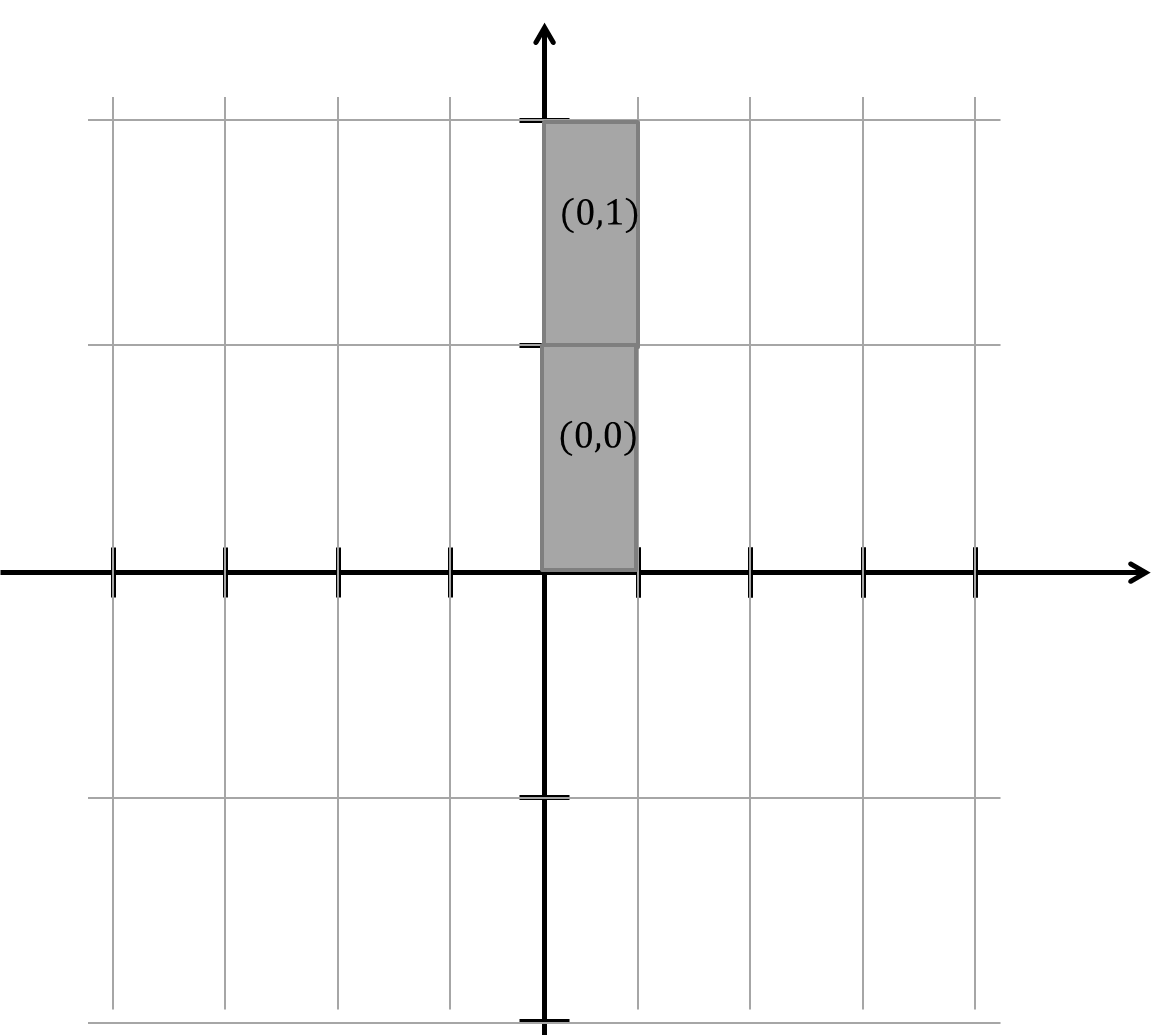
\includegraphics[scale=0.28]{Pics/example_hc_2d.png}
\label{fig:hcExample}
}\hspace{0.3cm}
\subfloat[The abstract state of \statement{px,py} after the first iteration of the loop (widths are, respectively, $10.0$ and $25.0$)]{
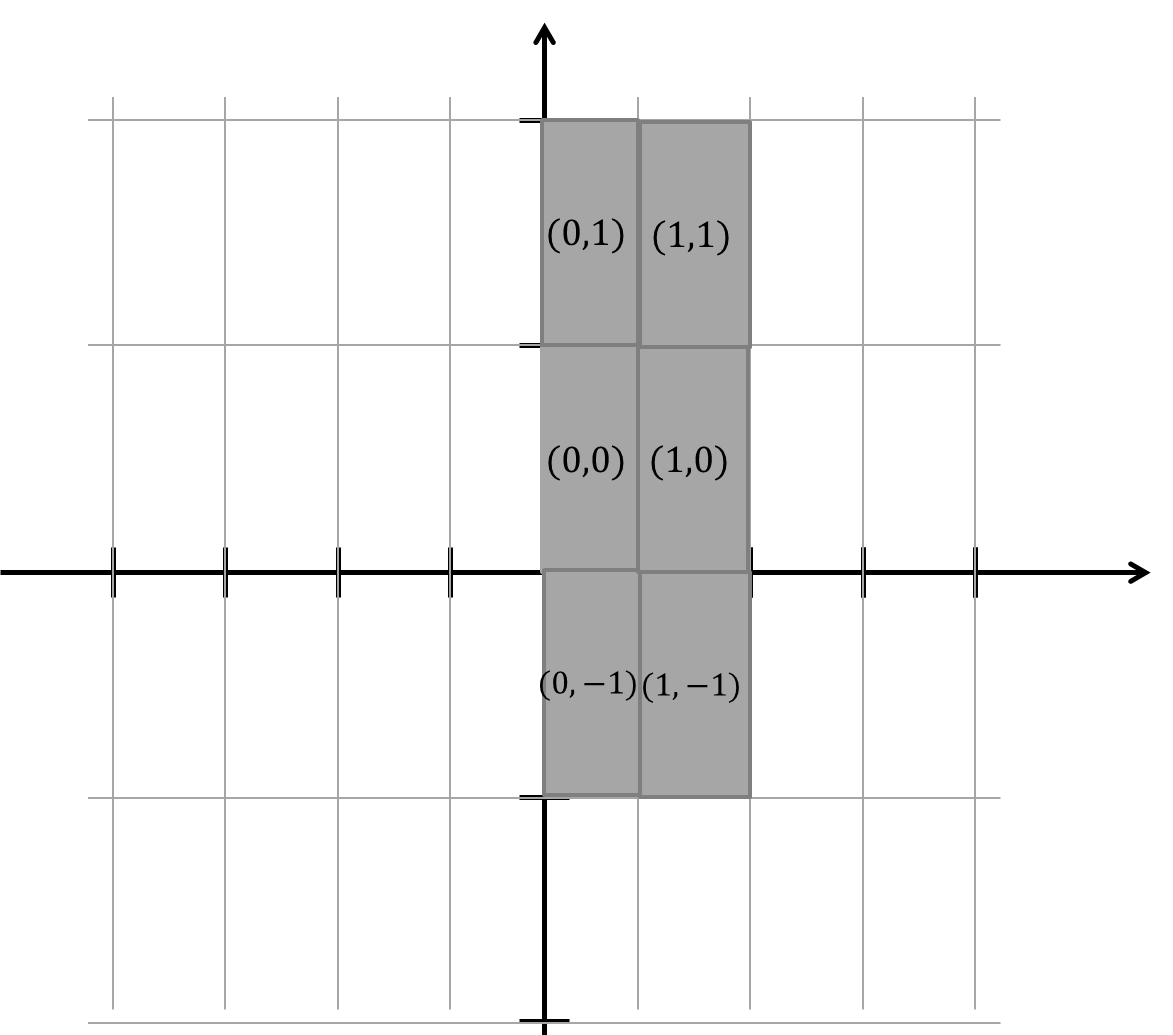
\includegraphics[scale=0.28]{Pics/example_hc_2d_2.png}
\label{fig:hcExample2}
}
\caption{Cartesian plans}
\end{figure}
\vspace{-10pt}


%\begin{figure}[ht]
%\begin{centering}
%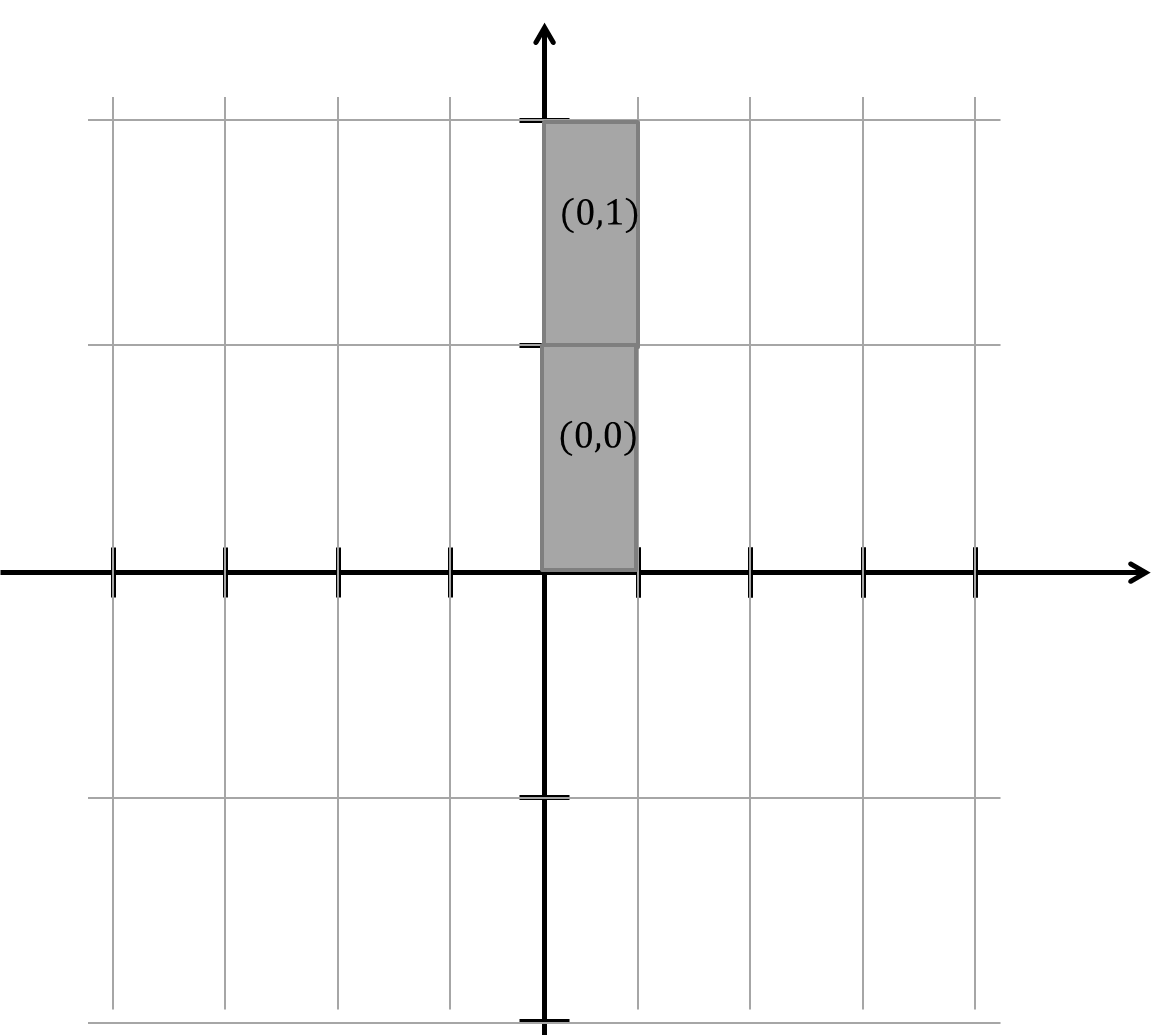
\includegraphics[scale=0.35]{Pics/example_hc_2d.png}
%\caption{The abstract state of the case study after the initialization of the variables (focusing the attention only on \statement{px,py}, when their widths are, respectively, $10.0$ and $25.0$)}
%\label{fig:hcExample}
%\end{centering}
%\end{figure}
%
%\begin{figure}[ht]
%\begin{centering}
%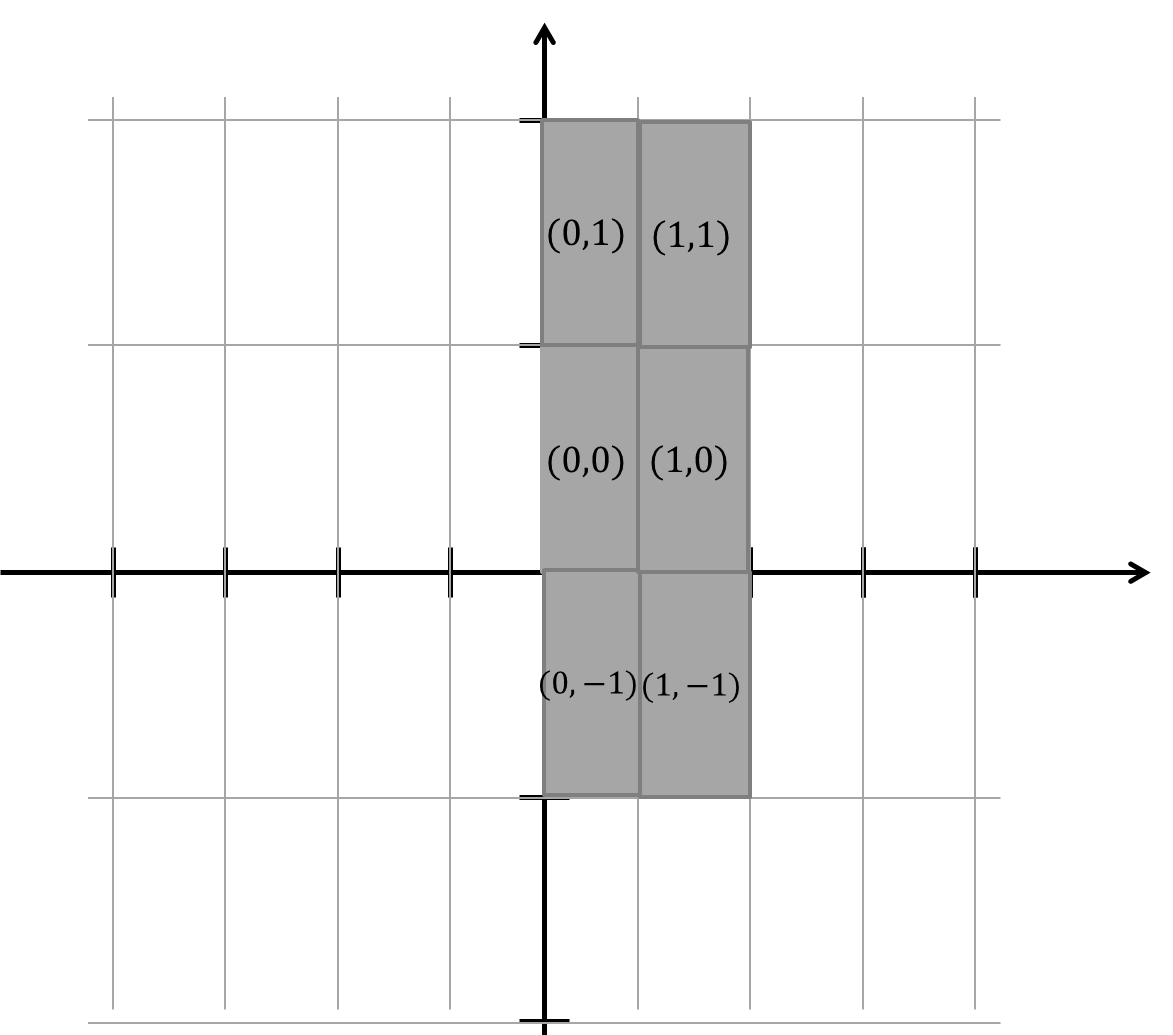
\includegraphics[scale=0.35]{Pics/example_hc_2d_2.png}
%\caption{The abstract state of the case study after the first iteration of the loop (focusing the attention only on \statement{px,py}, when their widths are, respectively, $10.0$ and $25.0$)}
%\label{fig:hcExample2}
%\end{centering}
%\end{figure}


We now formalize our abstract domain. Each abstract state is a set of hypercubes, where each hypercube is composed by $|\variables|$ integer numbers. The abstract domain is then defined by $\adomain = \wp(\integer^n)$ where $n = |\variables|$. The definition of lattice operators relies on set operators.
%: the partial order is defined through set inclusion, the lub and glb are set union and set intersection, respectively, while bottom and top are the empty set and the set containing all possible $n$-dimensional hypercubes, respectively. 
Formally, $\langle\wp(\integer^n), \subseteq, \cup, \cap, \emptyset, \integer^n\rangle$.

%\begin{lemma}
%$\langle\wp(\integer^n), \subseteq, \cup, \cap, \emptyset, \integer^n\rangle$ is a complete lattice.
%\begin{proof}
%The proof follows immediately by basic properties of set operators.
%\end{proof}
%\end{lemma}

\vspace{-10pt}
\subsection{Concretization function}
\vspace{-5pt}
We denote by $\agenericdomain$ the non-relational abstract domain on which our analysis is parameterized, and by $n$ the number of variables of the program. Let $\sigma \in \real^n$ be a tuple and $\sigma_i \in \real$ be the $i$-th element of such tuple. Also, let $\gamma_\agenericdomain : \funzione{\agenericdomain}{\wp(\real)}$ be the concretization function of abstract values of the non-relational abstract domain $\agenericdomain$, and $\function{getAbsValue}_v : \funzione{\naturals}{\agenericdomain}$ be the function that, given an integer index, returns the abstract value (in the domain $\agenericdomain$) which corresponds to that index inside the tuple $v$.
Then, the function $\gamma_{\aval} : \funzione{\wp(\agenericdomain^n)}{\wp(\real^n)}$ concretizes a set of hypercubes to a set of vectors of $n$ floating point values. Formally, $\gamma_{\aval}(\cel{V}) = \{\sigma : \exists v \in \cel{V} : \forall i \in [1..n] : \sigma_i \in \gamma_\agenericdomain(\function{getAbsValue}_v(i)) \}$ where $\cel{V} \in \wp(\agenericdomain^n)$ is a set of hypercubes.
Finally, based on $\gamma_{\aval}$, we can define the function $\gamma_{\adomain}$, which maps a subset $\cel{V}$ of $\wp(\agenericdomain^n)$ into an environment. The function $\gamma_{\adomain} : \funzione{\wp(\agenericdomain^n)}{\wp(\funzione{\variables}{\real})}$ concretizes the hypercubes domain. Formally, $\gamma_{\adomain}(\cel{V}) = \{[\statement{x} \mapsto \cel{\sigma}_{\avariableindex{\statement{x}}} : \statement{x} \in \variables] : \cel{\sigma} \in \gamma_{\aval}(\cel{V})\}$.  The function $\gamma_{\adomain}$ maps the vectors returned by $\gamma_{\aval}$ into concrete environments relying on the function $\avariableindexname : \funzione{\variables}{\naturals}$. The latter, given a variable, returns its index in the tuples which compose the elements of \adomain.

%Intuitively, we represent a concrete value as a tuple of real values (one for each variable of the program). The concretization of an abstract state $h \in \adomain$ is then a set of tuples. The concretization of $h$ is the union of all the concretizations of its hypercubes, i.e., all the points belonging to the volumes of its hypercubes. Each tuple of the concretization of $h$, then, is a point belonging to one hypercube of $h$. 

\vspace{-10pt}
\subsection{Convergence of the analysis}
\vspace{-5pt}
%The domain described so far does not ensure the convergence of the analysis. In fact, a \statement{while} loop may add new hypercubes with increased indices at each iteration, and the dimension of the abstract state (i.e., the hypercubes set) would increase at each iteration without converging. Thus, we need a way to force the convergence of the analysis. Given our abstract state representation, 
The number of hypercubes in an abstract state may increase indefinitely. In order to make the analysis convergent, we fix for each variable of the program a maximum integer index $n_i$ such that $n_i$ represents the interval $[n_i \times w_i .. +\infty]$. The same happens symmetrically for negative values. In this way, the set of indices of a given variable is finite, the resulting domain has finite height, and the analysis is convergent.

This approach may seem too rough since we establish the bounds of intervals before running the analysis. However, 
%this allows us to control the number of possible intervals in our hypercubes, and this is particularly important for the efficiency of the overall analysis. In addition, 
when analysing physics simulations we can use the initialization of variables and the property to verify in order to establish convenient bounds for the intervals. For instance, in the case study presented in Section \ref{sec:case_study} we are interested in checking if a ball stays in the screen, that is, if \statement{px} is greater than zero and less than a given value \statement{w} representing the width of the screen. Since we are only interested in proving that, once a ball has exited the screen, it does not come back, we can abstract together all the values that are greater than \statement{w}.

%Observe that more sophisticated widening operators could be used as an alternative to the adopted solution described above, but this could affect the performance of the resulting analysis.

%\subsection{Other data types or non-relational abstractions}
%\todogiulia{Secondo me questa subsection si puo' cancellare}
%As suggested before, for now we focus the application of our abstract domain to physics simulations, and for this reason we abstract floating point variables through intervals of fixed width. However, we may apply other kind of abstractions (e.g., the Sign domain) to our framework to consider other types of variables (integer, boolean, etc.). We will sketch other possible applications of our framework in Section \ref{sec:otherapplications}.

\vspace{-10pt}
\subsection{Offsets}
\vspace{-5pt}
A loss of precision may occur due to the fact that hypercubes proliferate too much, even using small widths. Consider, for example, the statement \statement{x = x + 0.01} (which is repeated at each iteration of the \statement{while} loop) with $1.0$ as the width associated to \statement{x}. If $[0.0 .. 1.0]$ was the initial interval associated to \statement{x}, the sequence of abstract states would be: $\{ [0.0 .. 1.0] \}$, $\{ [0.0 .. 1.0], [1.0 .. 2.0] \}$, $\{ [0.0 .. 1.0], [1.0 .. 2.0], [2.0 .. 3.0] \}$ and so on. At each iteration we would add one interval. 
%If the initial interval associated to \statement{x} was $[0.0 .. 1.0]$, after the first iteration we would obtain two intervals ($[0.0 .. 1.0]$ and $[1.0 .. 2.0]$) because the resulting interval would be $[0.01 .. 1.01]$, which spans over two fixed-width intervals. For the same reason, after the second iteration we would obtain three intervals ($[0.0 .. 1.0],[1.0 .. 2.0]$ and $[2.0 .. 3.0]$) and so on: at each iteration we add one interval. 

In order to overcome these situations, we further improve the definition of our domain: in each hypercube, each variable $v_i$ (associated to width $w_i$) is related to (other than an integer index $i$ representing the fixed-width interval $[i \times w_i .. (i+1) \times w_i]$) a specific offset $(o_m,o_M)$ \emph{inside} such interval. In this way, we use a sub-interval (of arbitrary width) inside the fixed-interval width, thereby restricting the possible values that the variable can assume. Both $o_m$ and $o_M$ must be smaller than $w_i$, greater than or equal to $0$ and $o_m \leq o_M$. Then, if $i$ and $(o_m,o_M)$ are associated to $v_i$, this means that the possible values of $v_i$ belong to the interval $[(i \times w_i) + o_m .. (i \times w_i) + o_M]$.

An element of our abstract domain is then stored as a map from hypercubes to tuples of offsets. In this way, we can keep the original definition of a hypercube as a tuple of integers, but we also map each hypercube to a tuple of offsets (one for each variable). Now an abstract state is defined by $M : \funzione{\integer^{|Vars|}}{{(\real \times \real)}^{|Vars|}}$, i.e., a map where the domain is the set of hypercubes, and the codomain is the set of tuples of offsets.

The least upper bound between two abstract states ($M=M_1 \sqcup M_2$) is then defined by $dom(M) = dom(M_1) \cup dom(M_2)$, and

$$
\forall h \in dom(M) : M(h) = \begin{cases}
M_1(h) & \mbox{if } h \in dom(M_1) \wedge h \notin dom(M_2) \\
M_2(h) & \mbox{if } h \in dom(M_2) \wedge h \notin dom(M_1) \\
merge(M_1(h),M_2(h)) & \mbox{otherwise }
\end{cases}$$
where $merge(o_1,o_2)$ creates a new tuple of offsets by merging the two tuples of offsets in input: for each pair of corresponding offsets (for example $(m_1,M_1)$ and $(m_2,M_2)$), the new offset is the widest combination possible (i.e., $(\min(m_1,m_2)$ and $\max(M_1,M_2))$). Note that this definition corresponds to the pointwise application of the least upper bound operator over intervals. The widening operator is extended in the same way: it applies the standard widening operators over intervals pointwisely to the elements of the vector representing the offsets.


\vspace{-10pt}
\section{Abstract semantics}
\vspace{-5pt}
\label{sec:semantics}
For the most part, the abstract semantics applies existing semantic operators of boxed Intervals \cite{COU98}. In this section, we sketch how these operators are used to define the semantics on \adomain.

First of all, $\mathbb{I}$ defines the semantics of arithmetic expressions on a single hypercube by applying the well-known arithmetic operators on intervals. 

We use the semantics $\mathbb{I}$ to define the abstract semantics $\mathbb{B}$ of Boolean comparisons. Given a hypercube and a Boolean comparison $E_1 <bop> E_2$ where $<bop> \in \{\geq, >, \leq, <, \neq \}$, $\mathbb{B}$ returns an \emph{abstract value of the boolean domain} (namely, $\mathit{true}$, $\mathit{false}$, or $\top$) comparing the intervals obtained from $E_1$ and $E_2$ through $\mathbb{I}$. Therefore, given a Boolean condition and a set of hypercubes, we partition this set into the hypercubes for which (i) the condition surely holds, (ii) the condition surely does not hold, and (iii) the condition may or may not hold. In this way, we can discard all the hypercubes for which a given Boolean condition surely holds or does not hold.
%Note that in this way we lose some precision. For instance, imagine that in a given hypercube we know that $\statement{x} \in [0..5]$ (because the fixed width of intervals associated to \statement{x} is 5), and we check if $\statement{x} \leq 3$. The answer of $\mathbb{B}$ will be $\top$ and, if the condition was inside an \statement{if} statement, this hypercube will be used to compute the semantics of both the branches. Indeed, we would know that $\statement{x} \in [0..3]$ in the \statement{then} branch, and $\statement{x} \in [4..5]$ in the else branch. Nevertheless, we cannot and do not want to track this information in our hypercube, since the width of the interval associated to \statement{x} is 5, and fixed widths are a key feature in order to obtain an efficient analysis. We will present (Section \ref{sec:widths}) how we can recursively modify the widths of the analysis to improve precision in these cases.\todopietro{Remove it when merging section 6 here - the details about the offset should be presented before and here we should report the formal definitions}
The semantics of the logical operators $not$, $and$, $or$ is defined in the standard way.

$\mathbb{I}$ is used to define the semantics $\mathbb{S}$ of variable assignment as well. The standard semantics of \statement{x=exp} is to (i) obtain the interval representing the right part ($\mathbb{I}\llbracket\statement{x=exp}, \sigma\rrbracket=[m..M]$), and (ii) assign it in the current state. This approach does not necessarily produce a single hypercube, since the interval to assign could have a greater width than the fixed width of the assigned variable (for example, the interval $[0..6]$ when $w=5$). It could also happen that the resulting interval width is smaller than the fixed width, but the interval spans over more than one hypercube side, due to the fixed space partitioning (for example, the interval $[3..6]$ when $w=5$, because the space is partitioned in $[0..5],[5..10]$, etc.). In these cases, we build up several hypercubes that cover the interval $[m..M]$. This can be formalized by $assign(h, V_i, [a..b])=\{h[i\mapsto m] : [m\times w_i .. (m+1)\times w_i]\cap [a..b] \neq \emptyset\}$, where $h$ is a hypercube, $V_i$ is the assigned variable, and $[a..b]$ is the interval we are assigning (which depends on the hypercube $h$, since we use its variables values to compute the result of the expression). We repeat this process for each hypercube $h$ in the abstract state by using it as input for the computation of $assign$.
In this way, we are able to over-approximate the assignment while also keeping the fixed widths of the intervals, which are very important for performance issues.

\vspace{-10pt}
\subsubsection{Offsets}
Offsets allow us to recover some precision when computing the abstract semantics of assignment. In particular, as the expression semantics $\mathbb{I}$ returns intervals of arbitrary widths, we can use such exact result to update the offsets of the abstract state. Formally, the semantics of the assignment is defined as follows: 
\begin{equation*}
assign(h, V_i, [a..b]) = \{ h[i\mapsto (m,o_m,o_M)] : [m\times w_i .. (m+1)\times w_i] \cap [a..b] \neq \emptyset \}
\end{equation*}
where $h$ is a hypercube, $V_i$ is the assigned variable, $[a..b]$ is the interval we are assigning and $o_m, o_M$ are computed as:
\begin{equation*}
o_m = \begin{cases} 
0 & \mbox{if } a \leq (m \times w_i) \\
a - (m \times w_i) & \mbox{otherwise} \\
\end{cases} \wedge 
o_M = \begin{cases} 
w_i & \mbox{if } b \geq ((m+1) \times w_i) \\
b - (m \times w_i) & \mbox{otherwise} \\
\end{cases}
\end{equation*}
Note that, when we extract from a hypercube the interval associated to a variable, we use the interval delimited by the offsets, so that abstract operations can be much more precise. 

Consider the evaluation of statement \statement{x = x + 0.01} inside a while loop with $1.0$ as width of \statement{x} and $[0..1]$ as initial value of \statement{x}. After the first iteration, the abstract semantics computes $[0.0 .. 1.0]$ and $[1.0 .. 2.0]$ with offsets $[0.01 .. 1.0]$ and $[1.0 .. 1.01]$, respectively. In this way, at the following iteration we would obtain again the same two intervals with the offsets changed to $[0.02 .. 1.0]$ and $[1.0 .. 1.02]$. This results is strictly more precise than the one obtained without offsets, and it is an essential feature of our abstract domain. For instance, in the case study of Figure \ref{lst:casestudy} offsets will allow us to discover if a bouncing ball exits the screen after $N$ iterations of the \statement{while} loop.

\vspace{-10pt}
\subsection{Initialization of the analysis} \label{sec:initialization}
\vspace{-5pt}
Before starting the analysis we have to determine the number of sides each hypercube will have. To do this, we must find all the variables ($Vars$) of the program which are not constants (i.e., assigned only once at the beginning of the program). %To avoid scanning the entire code before starting the analysis, 
We require the program to initialize all the variables at the beginning of the program. 
%Note that physics simulations, like our case study, satisfy this requirement because they are made up by an initialization of all variables, followed by a \statement{while} loop which contains the core of the program (i.e., the update of the simulated world). Otherwise, we can consider a dummy initialization (i.e., $0.0$) for all variables which are not initialized at the beginning of the program. The actual initialization of the variables will be treated as a normal assignment, without any loss of precision. 
The initialization of the analysis is made in two steps. First, for each initialized variable, we compute its abstraction in the non-relational domain chosen to represent the single variables. The resulting set of abstract values could contain more than one element. Let us call $\alpha(V)$ the set of abstract values associated to the initialization of the variable $V \in Vars$. Then we compute the Cartesian product of all sets of abstracted values (one for each variable). The resulting set of tuples (where each tuple has the same cardinality as $Vars$) is the initial set of hypercubes of the analysis. 
Formally, $\adomain = \sbigtimes_{V \in Vars} {\alpha(V)}$.

Consider the code of our case study in Figure \ref{lst:casestudy}. First of all, we must identify the variables which are not constants: $dt,g,k$ are assigned only during the initialization, so we do not include them in $Vars$. The set of not-constant variables is then $Vars = \{ V_1 = px, V_2 = py, V_3 = vx, V_4 = vy \}$, and so $|Vars| = 4$.
%Suppose that the widths associated to the variables are  $w_1 = 10.0, w_2 = 25.0, w_3 = 30.0, w_4 = 5.0$. Then, the abstraction of each variable is $\alpha(V_1) = \{ 0 \}$, $\alpha(V_2) = \{ 0, 1 \}$, $\alpha(V_3) = \{ 0, 1 \}$, and $\alpha(V_4) = \{ -6 \}$.
%The Cartesian product of these abstractions brings us to the following initial set of hypercubes:
%$$\adomain = \{ (0,0,0,-6) , (0,0,1,-6) , (0,1,0,-6) , (0,1,1,-6) \}$$

\vspace{-10pt}
\subsection{Tracking the origins}\label{sec:origins}
\vspace{-5pt}
During the analysis of a program we also track, for each hypercube of the current abstract state, the initial hypercubes (\textit{origins}) from which it is derived. To store such information, we proceed as follows. Let $H_i$ be the set of hypercubes obtained for the $i$-th statement of the program. The data structure of a hypercube $h$ contains also an additional set of hypercubes, $h^{or}$, which are its origins and are always a subset of the initial set of hypercubes, i.e., $\forall h : h^{or} \subseteq H_0$. At the first iteration, each hypercube contains only itself in its origins set: $\forall h \in H_0 : h^{or} = \{ h \}$. When we execute a statement of the program, each hypercube produces some new hypercubes: at this stage, the origins set is simply propagated. For example, if $h$ generates $h_1,h_2$, then $h_1^{or} = h_2^{or} = h^{or}$. When merging all the newly produced hypercubes in a single set (the abstract state associated to the point of the program just after the executed statement), we also merge through set union the sets of origins of any repeated hypercube. For example, consider $H_i = \{ h_a, h_b \}$ and let $h_1,h_2$ be the hypercubes produced by $h_a$ executing statement $i$-th and $h_2,h_3$ be those produced by $h_b$. Then, $H_{i+1} = \{ h_1,h_2,h_3\}$ and $h_1^{or} = h_a^{or}$, $h_2^{or}= h_a^{or} \cup h_b^{or}$ and $h_3^{or} = h_b^{or}$.

\vspace{-10pt}
\subsection{Width choice} \label{sec:widths}
\vspace{-5pt}
The choice of the interval widths influences both the precision and efficiency of the analysis. On the one hand, if we use smaller widths we certainly obtain more precision, but the analysis risks to be too slow. On the other hand, with bigger widths the analysis will be surely faster, but we could not be able to verify the desired property. To deal with this trade-off, we implemented a recursive algorithm which adjusts the widths automatically.
We start with wide intervals (i.e., coarse precision, but fast results) and we run the analysis for the first time. At the end of the analysis, we check, for each hypercube of the \emph{final} set, if it verifies the desired property. We then associate to each \emph{origin} (i.e., initial hypercube) its final result by merging the results of its derived final hypercubes (we know this relationship because of the origins set stored in each hypercube): some origins will certainly verify the property (i.e., they produce only final hypercubes which satisfy the property), some will not, and some will not be able to give us a definite answer (because they produce both hypercubes which verify the property and hypercubes which do not verify it). We partition the starting hypercubes set with respect to this criterion (obtaining, respectively, the \emph{yes} set, the \emph{no} set and the \emph{maybe} set), and then we run the analysis again with halved widths, but \emph{only} on the origins which did not give a definite answer (the \emph{maybe} set). This step is only performed until we reach a specific threshold, i.e., the \textit{minimum width} allowed for the analysis. The smaller this threshold is, the more precise (but slower) the analysis becomes.

%At the end of this recursive process, we obtain three partitions of the variable space: a set of starting hypercubes which certainly verify the property (\emph{yes} set), a set of starting hypercubes which certainly do not verify the property (\emph{no} set), and a set of starting hypercubes which, at the minimum width allowed for the analysis, still do not give a definite answer (\emph{maybe} set). 
The analysis is then able to tell us which initial values of the variables bring us to verify the property (the union of all the \emph{yes} sets encountered during the recursive algorithm) and which do not. Thanks to these results, the user can modify the initial values of the program, and run the analysis again, until the answer is that the property is verified \emph{for all initial values}. In our case study, for example, we can adjust the possible initial positions and velocities until we are sure that the ball will exit the screen in a certain time frame. 

The formalization of this recursive algorithm is presented in Algorithm \ref{alg:widthAdjusting}.

\begin{algorithm}
\caption{The width adjusting recursive algorithm} \label{alg:widthAdjusting}
\begin{algorithmic} 
\Function {Analysis} {$currWidth, minWidth, startingHypercubes$}
  \State \Return $(yes \cup yes', no \cup no', maybe')$
  \State \textbf{where}
    \State $(yes, no, maybe) = hypercubesAnalysis(currWidth, startingHypercubes )$
    \If {$currWidth/2.0 \geq minWidth$}
      \State $(yes', no', maybe') = Analysis(currWidth/2.0, minWidth, maybe)$
    \Else
      \State $(yes', no', maybe') = (Set.empty, Set.empty, maybe)$
    \EndIf
\EndFunction
\end{algorithmic}
\end{algorithm}

%The overall analysis takes as input the starting width, the minimum width allowed and the set of starting hypercubes (obtained from the initialization of the program as described in Section \ref{sec:initialization}). It executes the analysis on such data with the function \statement{hypercubesAnalysis}, which returns three sets of hypercubes (\statement{yes,no,maybe}) with the meaning explained above. Then, if the halved width is still greater than the minimum one allowed, the algorithm performs a recursive step by repeating the analysis function only on the \statement{maybe} hypercubes set (with halved width). 

%Note that %the initial hypercubes sets 
%the three final hypercubes sets (the \emph{yes,no,maybe} partitions)
%will contain hypercubes of different sizes: this happens because each hypercube can come from a different iteration of the analysis, and each iteration is associated to a specific hypercube size. A certain portion of the variable space could give a definite answer even at coarse precision (for example, when the horizontal velocity of the ball is sufficiently high, the values of other variables do not matter so much), while another portion could need to be split in much smaller hypercubes to give interesting results.

%\todogiulia{Tino: come dicevo questa sezione si dovrebbe ridurre all'osso: riferimenti a Intervalli, Disjuctinve domains trough Powerset, Prodotto Cartesiano, Conditional Partitioning}
%
%In this Section, we define the abstract semantics of Hypercubes. In particular, the semantics we will define are the following ones:
%\begin{itemize}
%\item $\mathbb{I}$, the abstract semantics of arithmetic expressions, which receives an expression and a single hypercube in input and returns an \emph{interval of real values} resulting from the execution of that expression when the variable values belong to that hypercube.
%\item $\mathbb{B}$, the abstract semantics of boolean conditions, which receives a single hypercube and two expressions in input and returns an \emph{abstract value of the boolean domain} (namely, $true$, $false$, or $\top$) obtained by comparing the two expressions (through $\geq, >, \leq, <$ or $\neq$) when the variable values belong to that hypercube. Boolean conditions can be combined through logical operators (and, or, not) in the usual way (i.e., exploiting the abstract semantics of the boolean abstract domain). 
%\item $\mathbb{S}$, the abstract semantics of statements, which receives in input a set of hypercubes (the current abstract state) and returns a new set of hypercubes (the new abstract state after the execution of the statement).
%\end{itemize}
%
%\subsection{The abstract semantics of arithmetic expressions, $\mathbb{I}$}
%
%\subsubsection{Constants}
%\label{sec:constants}
%We define a constant as a variable which gets assigned only once with a constant value, or a numerical value which appears in some statements (without being assigned to a specific variable). To simplify the treatment of constants, we execute a preprocessing on the program with constant propagation, to remove constant variables and replace their uses with their numerical value. 
%
%
%The abstract semantics of an expression made up by a constant numeric value is, simply, an interval of zero width: the extremes of the interval are the same and they are equal to the value of the constant. 
%Then, the abstract semantics of a constant is:
%
%$$\mathbb{I}\llbracket c \rrbracket \; h = [c,c]$$
%
%Note that the value of the hypercube in input ($h$) is i,nored because it is not needed to compute the result.\ nn
%
%\subsubsection{Intervals}
%The abstract semantic of an expression made up by an interval of real values is immediate: it is exactly that interval, without modifications. We ignore the hypercube passed in input.
%
%$$\mathbb{I}\llbracket (m,M) \rrbracket \; h = [m,M]$$
%
%\subsubsection{Variables}
%When the expression is made up by a variable, we must consider the abstract value of that variable in the hypercube passed in input. Let $h_i$ be the integer index associated to the $i$-th dimension of the hypercube, $V_i$ the $i$-th variable defined in the program and $w_i$ the width associated in the analysis to such variable. Then, the abstract semantics of a variable  is $\mathbb{I}\llbracket V_i\rrbracket \; h = [h_i*w_i,(h_i+1)*w_i]$.
%
%
%\subsubsection{Arithmetic operations}
%We considered only the most used arithmetic operators. In particular, we considered sum ($+$), subtraction ($-$), product ($\times$) and division ($\div$). These operators should suffice for most physics simulations (for example, our case study requires only sum and product - the change of sign being a multiplication for $-1$). Anyway, our framework can be easily extended to support other operations (for example modulus), by simply defining their abstract semantics when working on intervals of values.
%
%The semantics of these operators over intervals has been already deeply studied, and we refer to \cite{COU98} for their definitions.
%
%
%\subsection{The abstract semantics of Boolean conditions, $\mathbb{B}$}
%\label{sec:boolcondition}
%We now define the semantics of integer comparison using the operators $>$, $<$, $\leq$, $\geq$, and $\neq$. 
%
%The abstract semantics separately computes the semantics on the left and right arithmetical expressions of the statement, obtaining two intervals. Let us call them $i_1 = [a,b]$ and $i_2 = [c,d]$. The abstract comparison between them depends on the specific comparison operator present in the statement:
%\begin{itemize}
%\item $i_1 \neq i_2$ returns true if $b < c \vee a > d$, false if $b=c=a=d$, and $\top$ otherwise.
%\item $i_1 < i_2$ returns true if $b < c$, false if $a > d$, top otherwise.
%\item $i_1 > i_2$ returns true if $a > d$, false if $b < c$, top otherwise.
%\item $i_1 \leq i_2$ returns true if $b \leq c$, false if $a \geq d$, top otherwise.
%\item $i_1 \geq i_2$ returns true if $a \geq d$, false if $b \leq c$, top otherwise.
%\end{itemize}
%
%$\mathbb{B}$ will be used by the statement semantics $\mathbb{S}$ when computing the semantics of \statement{if} and \statement{while} statements to discard the hypercubes that surely do not satisfy the condition. Note that in this way we lose some precision. For instance, imagine that in a given hypercube we know that $\statement{x} \in [0..5]$ (because the fixed width of intervals associated to \statement{x} is 5), and we check if $\statement{x} \leq 3$ when computing the semantics of an \statement{if} statements. The answer of $\mathbb{B}$ will be $\top$, and so this hypercube will be used to compute the semantics of both the branches. Indeed, we would know that $\statement{x} \in [0..3]$ in the \statement{then} branch, and $\statement{x} \in [4..5]$ in the else branch. Nevertheless, we cannot track this information in our hypercube, since the width of the interval associated to \statement{x} is 5. Anyway, we will present (Section \ref{sec:widths}) how we can recursively modify the widths of the analysis to improve precision in these cases.
%
%
%\subsection{The abstract semantics of statements, $\mathbb{S}$}
%
%\subsubsection{Assignment}
%Usually, with non-disjunctive domains, the abstract semantics of an assignment is straightforward: you have to compute the abstract semantics of the expression and update the abstract value of the variable with the result. In our domain, though, we track a different kind of information: we represent possible values of all variables together (through hypercubes) and we consider disjunctive information (a set of valid hypercubes instead of a single hypercube). Therefore, we must devise a specific abstract semantics to deal with the assignment statement. 
%
%Let the assignment be $V_i = e$, where $e$ is an arithmetic expression. Our approach can then be sketched as follows: 
%\begin{itemize}
%\item we consider, separately, each hypercube $h$ of the current state;
%\item we compute the abstract semantics of the arithmetic expression $e$ passing to it the hypercube $h$.
%\item we create a new hypercube (or \emph{some} new hypercubes, depending on the width of the resulting interval), where the abstract value of $V_i$ is the abstraction of the interval resulting from $e$.
%\end{itemize}
%
%If the interval obtained from $e$ overlaps over several partitions established for variable $V_i$, we have to build up several hypercubes as result of the assignments semantics over a single hypercube. 
%
%
%On the other hand, if many hypercubes of the initial state map to the same hypercube in the resulting state, it could also happen that the cardinality of \adomain\ decreases (or remains unmodified) after the execution of an assignment.
%
%Formally: 
%
%$$\mathbb{S}\llbracket \statement{V_i = e}\rrbracket \; H = \bigcup_{h \in H} {assign(h, V_i, \mathbb{I}\llbracket e\rrbracket \; h)}$$
%
%where $assign(h, V_i, [a,b])=\{h[i\mapsto m] : [m\times w_i .. (m+1)\times w_i]\cap [a..b] \neq \emptyset\}$. The output of this function is the set of hypercubes covering all the intervals that overlaps with the interval assigned to the given variable.
%
%
%\subsubsection{If-then-else semantics}
%
%To precisely deal with branches of \statement{if} statements, we partition the abstract state \adomain\ with respect to the evaluation of the branching condition. In particular, we compute the abstract semantics $\mathbb{B}$ of the boolean condition on each hypercube of \adomain\ and we assign each hypercube to a specific partition, based on the result of the condition semantics. Therefore, we obtain three partitions: the hypercubes for which the condition evaluates to true ($p_t$), the ones for which the condition evaluates to false ($p_f$), and the ones for which we do not have a definitive answer ($p_\top$).
%
%Once obtained these three partitions, we can compute selectively the abstract semantics of the two branches, and in particular the \statement{then} branch with $p_t \cup p_\top$, and the \statement{else} branch with $p_f \cup p_\top$. 
%
%Formally, the semantics of the \statement{if} statements follows:
%
%$$\mathbb{S}\llbracket \statement{if}(B)\ \statement{then}\ P_1\ \statement{else}\ P_2\rrbracket \; H = ( \mathbb{S}\llbracket P_1\rrbracket \; (p_t \cup p_\top) ) \cup ( \mathbb{S}\llbracket P_2\rrbracket \; (p_f \cup p_\top) )$$
%
%where $p_t = \{ h \in H : \mathbb{B}\llbracket \ael{if}\rrbracket \; h = true \}$, $p_f = \{ h \in H : \mathbb{B}\llbracket \ael{if}\rrbracket \; h = false \}$, and $p_\top = \{ h \in H : \mathbb{B}\llbracket \ael{if}\rrbracket \; h = \top \}$.
%
%\subsubsection{Concatenation of statements}
%The abstract semantics of the concatenation of two statements is straightforward: it executes the abstract semantics of the first statement, it takes the result and it passes it as input to the abstract semantics of the second statement. Formally:
%
%$$\mathbb{S}\llbracket P_1;P_2\rrbracket \; H = \mathbb{S}\llbracket P_2\rrbracket \; (\mathbb{S}\llbracket P_1\rrbracket \; H)$$
%
%\todogiulia{Non sono per niente convinto che sia questa big-step semantics quello di cui abbiamo bisogno. Ad esempio, la semantics di \statement{while(true) P_1; P_2} ritorna $\emptyset$ stando a questa definizione. A occhio abbiamo bisogno di qualcos'altro, e.g., uno stato astratto per ogni punto di programma di un cfg? In questo caso, non dobbiamo lavorare a questo livello con \statement{if} e \statement{while} ma piu' a basso livello.}
%
%\subsection{While loop}
%To do. 



\vspace{-10pt}
\section{Experimental results}
\vspace{-5pt}
\label{sec:experimental}
In this Section we present some experimental results on the case study presented in Section \ref{sec:case_study}. We want to check if \emph{Property 1} is verified on the program of Figure \ref{lst:casestudy} and, in particular, we want to know which subset of starting values brings to verify it.
We implemented our analysis in the \FSharp\ language with Visual Studio 2012. We ran the analysis on an Intel Core i5 CPU 1.60 GHz with 4 GB of RAM, running Windows 8 and the \FSharp\ runtime 4.0 under .NET 4.0. 

We set the initial widths associated to all variables to $100.0$ and the minimum width allowed to $5.0$. As for \emph{Property 1}, we set $T = 5$, i.e., we want to verify if the ball is surely out of the screen within $5$ seconds from its generation. Since $dt=0.05$, a simulation during $5$ seconds corresponds to $5/0.05 = 100$ iterations of the \statement{while} loop. To verify this property, we apply trace partitioning \cite{MR05} to track one abstract state per loop iteration until the 100-th iteration (we do not need to track precise information after the 100th iteration). The position which corresponds to the exiting from the screen is $100.0$: if after $100$ iterations the position \statement{px} is surely greater than $100.0$, then \emph{Property 1} is verified. The whole of these values (starting variables values and widths, minimum width allowed, number of iterations, position to reach) make up our \emph{standard workbench data}. We will experiment to study how efficiency and precision change when modifying some parameters of the analysis.
%, and for each test we will specify only the values which are different with respect to the standard workbench data.
%We will start by running the analysis on the standard workbench data, and then we will experiment by changing one value at a time to study how the efficiency and precision change\footnote{}. 

%For example, we will start by showing how precision and performance are affected by changing the minimum width allowed. After that, we will concentrate on the horizontal velocity variable and we will show how we can use our analysis as a form of \textquotedblleft assisted debugging\textquotedblright\ to understand which starting values of a variable bring to verify the property and which not. 

For each test, the analysis returns three sets of starting hypercubes: the initial values of the variables which satisfy the property (\textit{yes} set), which surely do not satisfy the property (\textit{no} set), and which may or not satisfy the property (\textit{maybe} set). To make the results more immediate and clearer, we computed for each \emph{yes} and \emph{no} set the corresponding volume covered in the space by their hypercubes. We also consider the \emph{total} volume of the variable space, i.e., the volume covered by all possible values with which the program variables are initialized. In the case of the standard workbench data, the \emph{total} volume is $10.0 \times 50.0 \times 60.0 \times 5.0 = 150000$. Dividing the sum of \emph{yes} and \emph{no} volumes by the \emph{total} volume, we obtain the percentage of the cases for which the analysis gives a definite answer. We will call this percentage the precision of the analysis. 

%Note that the \emph{total} volume refers to the initial variable space, i.e., to the space defined by the intervals assigned to the variables at the beginning of the program. The \emph{yes}, \emph{maybe}, and \emph{no} volumes refer to the same space, since they are defined in terms of \emph{starting} hypercubes. These volumes are all finite, since we suppose that all the variables are initialized by a bound interval, and this is always the case in Computer Games Software.

\subsubsection{Varying the minimum width allowed}
First of all, we run the analysis modifying the \emph{minimum width allowed} (MWA) parameter and we reported the results of these tests in Table \ref{table:minWidthAllowed}. We can clearly see the trade-off between performance and precision. %that the performance decreases when we set small widths, and it is instead very good on bigger ones. On the other hand, by decreasing the MWA we also gain more precision. 

\vspace{-15pt}
\begin{table}[ht]
\scriptsize
\caption{Varying the minimum width allowed (MWA)}
\centering 
\begin{tabular}{| c | c | c | c |}
\hline
MWA & Time (sec.) & \emph{yes+no} volume & Precision \\ \hline
3 & 530 & 131934 & 88\%  \\ %\hline 
5 & 77 & 99219 & 66\%  \\ %\hline 
12 & 11 & 40625 & 27\%  \\ %\hline 
24 & 1 & 25000 & 17\% \\ %\hline 
45 & 0.2 & 0 & 0\% \\ \hline 
\end{tabular}
\label{table:minWidthAllowed} 
\end{table}
\vspace{-30pt}

%\begin{figure}
%\begin{center}
%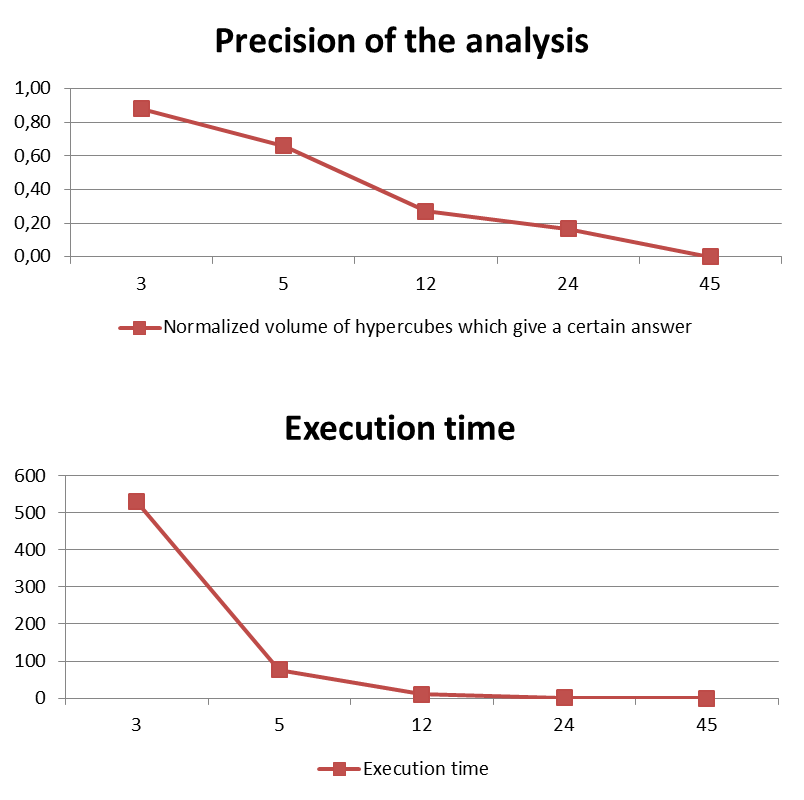
\includegraphics[scale=0.6]{Pics/varyingMWA.png}
%\caption{Varying the minimum width allowed - Plots}
%\label{fig:minWidthAllowed}
%\end{center}
%\end{figure}

%From these results,  For instance, when MWA = 45 we do not have any certain answer, while with MWA = 3 the certain answers cover the 88\% of the volume space, a quite precise result. 

\subsubsection{Finding appropriate starting values}

In Table \ref{table:velocityX} we reported the results of a series of successive tests obtained by changing the horizontal velocity of the ball (\statement{vx}). In particular, we made up a series of tests simulating the behavior of a developer using our analysis to debug his code. Let us suppose that we wrongly inserted a starting interval of negative values (between -120 and 0) for the horizontal velocity. The first test (\# 1) shows us that the program does not work correctly, since the \emph{no} volume is 100\%. Also, to give this answer, the analysis is very quick because a low MWA (45) suffices. After that, we try (test \# 2) with very high positive velocities (between 60 and 120) and we obtain (also very quickly) a 100\% of positive answer: we know for sure that with these velocities the program works correctly. Now it remains to verify what happens with velocities between 0 and 60, and we try this in test \# 3, where we decrease the MWA because we need more precision (the results with greater MWA were presented by the previous Section). Some values of \statement{vx} (i.e., $\geq 31.25$) ensure that the property is verified, some other values (i.e., $\leq 12.5$) ensure that the property is not verified, but the ones in between are uncertain. Tests \# 4 and \# 5 are just double checks.
%To do a double check about this data, we execute also tests \# 4 and \# 5, where we keep, respectively, only the low (between 0 and 15) and the high (between 30 and 60) values: in both cases the analysis is fairly quick in confirming the 100\% \emph{no} and 100\% \emph{yes}. 
So we try with a smaller MWA (3) in test \# 6 on the interval $[15..30]$: about a quarter of the starting values produces \emph{yes} and another quarter produces \emph{no}. The \emph{no} derives from low values (smaller than 18) and we confirm this in test \# 7. %, where (with a MWA of 5 and quick execution time) we obtain a 100\% of \emph{no} answers. 
As for medium-high values, test \# 6 shows that, with a velocity greater than 25, the answer is \emph{almost} always \emph{yes}. It is not always yes because, with this range of velocities, the values of other variables become important to verify the property. Test \# 8, in fact, shows us that velocities within 25 and 30 produce an 82\% of \emph{yes}, but a 18\% of \emph{maybe} remains. Finally, in test \# 9 we modify also other two variables (with values chosen looking at the results from test \# 6 and \# 8)
%: in particular, we set the horizontal position (\statement{px}) between 5 and 10, and the vertical position (\statement{py}) between 40 and 50. 
and, with such values, the answers are 100\% \emph{yes}. 

After these tests, the developer of the case study is sure that horizontal velocities below 18 will certainly not make the program work. On the other hand, values greater than 30 certainly make the program work. For values between 25 and 30, other variable values must be changed (\statement{px} and \statement{py}) to make the program work correctly. Making some other tests, we could also explore what happens with values between 18 and 25. 

\begin{table}[ht]
\scriptsize
\caption{Varying the horizontal velocity (\statement{vx})}
\centering 
\begin{tabular}{| l | c | c | c | l | p{5cm} |}
\hline
Test & \statement{vx} interval & MWA & Time (sec) & Answer & Comment \\ \hline
\# 1 & [-120 .. 0] & 45 & 1 & \emph{no} = 100\% & With negative values the answer is always no. \\ \hline 
\# 2 & [60 .. 120] & 45 & 0.2 & \emph{yes} = 100\% & With very high positive values the answer is always yes. \\ \hline 
\# 3 & [0 .. 60] & 5 & 77 & 
$\begin{array}{l}
\emph{yes} = 45\%\\
\emph{no}  = 21\%
\end{array}$ & Uncertainty. High values ($\geq$ 31.25) imply \emph{yes}, low values ($\leq$ 12.5) imply \emph{no}. \\ \hline 
\# 4 & [0 .. 15] & 24 & 0.5 & \emph{no} = 100\% & Double check on low values: answer always no. \\ \hline 
\# 5 & [30 .. 60] & 5 & 30 & \emph{yes} = 100\% & Double check on medium-high values: answer always yes. \\ \hline 
\# 6 & [15 .. 30] & 3 & 526 &
$\begin{array}{l}
\emph{yes} = 27\%\\
\emph{no} = 25\%
\end{array}$ & Uncertainty. Low values ($\leq$ 18) imply \emph{no}, for high values ($\geq$ 25) depends also on other variables. \\ \hline 
\# 7 & [15 .. 18] & 5 & 7 & \emph{no} = 100\% & Double check on medium-low values: answer always no. \\ \hline 
\# 8 & [25 .. 30] & 3 & 164 & 
$\begin{array}{l}
\emph{yes} = 82\%\\
\emph{maybe} = 18\%
\end{array}$ & Double check on medium-high values: answer almost always yes. In this case, also values of other variables influence the result. \\ \hline 
\# 9 & [25 .. 30] & 5 & 1 & \emph{yes} = 100\% & Modified also py ([40 .. 50]) and px ([5 .. 10]). Answer always yes. \\ \hline 
\end{tabular}
\label{table:velocityX} 
\end{table}
\vspace{-10pt}

\subsubsection{Discussion}
In this scenario, we ran the analysis by manually changing the initial values of program variables. Notice that this process could be automatized. 
%In particular, instead of providing a program that initializes all the variables, and checking if a given property holds, a user could give only the \statement{while} loop that performs the physics simulation, and then try wide ranges of initial values for the variables. This will obviously lead to an analysis that, even with large widths, could quickly give definite answers for a wide part of the given starting intervals. 
This process can be highly interactive, since the tool could show to the user even partial results while it is automatically improving the precision by adopting narrower intervals on the \emph{maybe} portion as described by Algorithm \ref{alg:widthAdjusting}. In this way, the user could iterate the process until it finds suitable initial values.

The execution times obtained so far underline that the analysis is efficient enough to be the basis of practical tools. Moreover, the analysis could be parallelized by running in parallel the computation of the semantics for each initial hypercube: exploiting several cores or even running the analysis in the cloud, we could further improve the efficiency of the overall analysis.
%. In this way, when we choose a narrow width, we could exploit several cores or even run the analysis in the cloud, thus improving the efficiency of the overall analysis.



\vspace{-10pt}
\section{Related work}
\vspace{-5pt}
\label{sec:related}
Various numerical domains have been studied in the literature, and they can be classified with respect to a number of different dimensions: finite (e.g., \textit{Sign}) versus infinite (e.g., \textit{Intervals}) height, relational (e.g., Octagons \cite{MIN06}) versus non-relational (e.g., \textit{Intervals}), convex (e.g., Polyhedra \cite{CH78}) versus possibly non-convex (e.g., donut-like domains \cite{G12}). Hypercubes track disjunctive information relying on Intervals. Similarly, the powerset operator \cite{FR99} allows one to track disjunctive information, but the complexity of the analysis grows up exponentially. Instead, we designed a specific disjunctive domain that reduces the practical complexity of the analysis by adopting indexes and offsets. 

%A number of different numerical abstract domains have been studied in the literature, and they can be classified with respect to a number of different dimensions: finite versus infinite height, relational versus non-relational, convex versus possibly non-convex, and so on. 
%
%The computational cost increases when lifting from finite non–relational domains like \textit{Sign} or \textit{Parity}, to 
%infinite non–relational domains like \textit{Intervals}, to sophisticated infinite relational domains like \textit{Octagons} \cite{MIN06}, \textit{Polyhedra} \cite{CH78}, \textit{Pentagons} \cite{LF08}, and \textit{Stripes} \cite{F08}, or to donut-like non-convex domains \cite{G12}. Moreover, when considering possibly non-convex disjunctive domains, as obtained through the powerset operator \cite{FR99}, the complexity of the analysis is growing (as well as its accuracy) in a full orthogonal (exponential) way. 

Noticeable efforts have been put both to reduce the loss of precision due to the upper bound operation, and to accelerate the convergence of the Kleene iterative algorithm \cite{HMG06,SB13,SISG06,BHZ07}, but they do not track disjunctive information.

%Noticeable efforts have been put both to reduce the loss of precision due to the upper bound operation, and to accelerate the convergence of the Kleene iterative algorithm. Some ways to reduce the space dimension in polyhedra computations relying on variable elimination and Cartesian factoring are introduced in \cite{HMG06}.  
%Seladji and Bouissou \cite{SB13} designed refinement tools based on convex analysis to express the convergence of convex sets using support functions, and on numerical analysis to accelerate this convergence applying sequence transformations. 
%On the other hand, Sankaranarayanan et al. \cite{SISG06} faced the issue of reducing the computational cost of the analysis using a powerset domain, by adopting restrictions based on \textquotedblleft on the fly elaborations\textquotedblright\ of the program's control flow graph. Efficiency issues about convergence acceleration by widening in the case of a powerset domain have been studied by Bagnara et al. in \cite{BHZ07}. All these domains do not track disjunctive information.

The trace partitioning technique designed by Mauborgne and Rival \cite{MR05} provides automatic procedures to build suitable partitions of the traces yielding to a refinement that has great impact both on the accuracy and on the efficiency of the analysis. This approach tracks disjunctive information, and it works quite well when the single partitions are carefully designed by an expert user. Unluckily, given the high number of hypercubes tracked by our analysis, this approach is definitely too slow for the scenario we are targeting.

Our spatial representation and width adjustment resembles the hierarchical data-structure of quadtrees in \cite{HKL10}. However, this paper contains only a preliminary discussion of the quadtree domain, and as far as we know it has not been further developed nor applied. %the authors are ``neutral" to the applicability of quadtrees for use in practical analyzers. 
Moreover, their domain is targeted to analyse only machine integers %(while we deal with real values) 
and the width is the same in each spatial axis. %(while we use a different width for each variable and offsets). %also, no offsets!

Our self-adaptive parametrization of the width shares some common concepts with  the CounterExample Guided Abstraction Refinement (CEGAR) \cite{CGJ00}. CEGAR begins checking with a coarse (imprecise) abstraction of the system and progressively refines it, based on spurious counterexamples seen in prior model checking runs. The process continues until either an abstraction proves the correctness of the system or a valid counterexample is generated. 
%This tool targets model checking systems, and it refines the level of abstraction by looking to a counter-example.

\cite{GC10} introduced the Boxes domain, a refinement of the Interval domain with finite disjunctions: an element of Boxes is a finite union of boxes. Each value of Boxes is a propositional formula over interval constraints and it is represented by the Linear Decision Diagrams data structure (LDDs). Note that the size of an LDD is exponential in the number of variables. We use a fixed width and a fixed partitioning on each hypercube dimension, while they do not employ constraints of this kind. In addition, Boxes uses a specific abstract transformer for each possible operation (for example, distinguishing $x = x + v$, $x = a \times x$, $x = a \times y$ and also making assumptions on the sign of constants) while our definitions are more generic. Finally, Boxes' implementation is based on the specific data structure of LDDs and cannot be extended to other base domains. %, while our approach can. 

%The Parametric Hypercubes proposal presented in this paper can be seen as a selection and a combination of most of these techniques, tailored to get a solution that properly suits the features of Computer Games Software applications. In this scenario, we had to track precisely a lot of disjunctive information. Therefore, we needed to introduce a targeted domain \adomain\ for physics simulations. On the other hand, some of the domain's features (like width parameter tuning, and interval offsets) may also be applied in other domains. 

If on the one hand Parametric Hypercubes have been tailored to Computer Games Software applications, on the other hand some of their features may also be applied to other contexts. In particular, our definition of  Computer Games Software applications (i.e., an infinite reactive loop, a complex state space with many real-valued variables, and strong dependencies among variables) exactly matches that of real-time synchronous control-command software (found in many industries such as aerospace and automotive industries). Hybrid systems and hybrid automata have been widely applied to verify this software. The formal analysis of large scale hybrid systems is known to be a very difficult process \cite{AHLP00}. In general, existing approaches suffer from performance issues or limitations on the property to prove, on the shape of the program, etc. For instance, \cite{BMC12} deals a simpler example than ours (a bouncing ball with only vertical motion) and in their benchmarks the variable space is quite limited: the velocity is a fixed constant, and the starting position varies only between 10 and 10.1. Instead, our Hypercubes can deal with velocities and positions bound inside any intervals of values. Also in \cite{B09} the variable space is more restricted than in our approach. 
%happens the same: the benchmark \emph{Heater} works on the variable space $[0..5]$, the \emph{Navigation} one on $[3.5..3.6] \times [3.5..3.6]$ and the \emph{Two-tanks} on $[5..5] \times [6..6]$; 
In addition, this analysis returns an abstraction of the final state of the program, while we also give information about which starting values are responsible for the property verification and which not.
%In \cite{HHW97} a lot of benchmarks are cited but no table with results and performances is presented. 
%\cite{ACH95} presents a general framework for the formal specification and algorithmic analysis of hybrid systems, while we proposed a specific analysis. 
\cite{HRP94} presents an application of the abstract interpretation by means of convex polyhedra to hybrid systems. This work is focused on a particular class of hybrid systems (\emph{linear} ones), and it is able to represent only convex regions of the space, since it employs the convex hull approximation of a set of values. \cite{ADI02} presents algorithms and tools for reachability analysis of hybrid systems by relying on predicate abstraction and polyhedra. However, this solution suffers from the exponential growth of abstract states and relies on expensive abstract domains. Finally, \cite{RS05} concerns safety verification of non-linear hybrid systems, starting from a classical method that uses interval arithmetic to check whether trajectories can move over the boundaries in a rectangular grid. This approach is similar to ours in the data representation (boxes). However, they do not employ any concept of offset, their space partitioning is not fixed and the examples they experimented with cover a very limited variable space.



\vspace{-10pt}
\section{Conclusions and future work}
\vspace{-5pt}
\label{sec:conclusions}
In this paper we presented Parametric Hypercubes, a disjunctive non-relational abstract domain which can be used to analyse physics simulations. Experimental results on a representative case study show the precision of the approach. The performance of the analysis makes it feasible to apply it in practical settings. 

Note that our approach offers plenty of venues in order to improve its results, thanks to its flexible and parametric nature. In particular, we could: (i) increase the precision by intersecting our hypercubes with arbitrary bounding volumes which restrict the relationships between variables in a more complex way than the offsets presented in Section \ref{sec:semantics}; (ii) increase the performance of Algorithm \ref{alg:widthAdjusting} by halving the widths only on some axes, chosen through an analysis of the distribution of hypercubes in the \emph{yes,no,maybe} sets; and (iii) study the derivative with respect to time of the iterations of the main loop in order to define temporal trends to refine the widening operator.
In addition, our domain is modular w.r.t. the non-relational abstract domain adopted to represent the hypercube dimensions. By using other abstract domains it is possible to track relationships between variables which do not necessarily represent physical quantities.

\bibliographystyle{plain}
\bibliography{Sections/10_references}

%\cite{}

\end{document}
